% !TeX spellcheck = en_US
\documentclass[hidelinks, english]{article}
\usepackage{etex}
\usepackage{microtype}
\usepackage{babel}
\usepackage[utf8]{inputenc}
\usepackage[T1]{fontenc}
\usepackage{graphicx}
\usepackage{listings}
\usepackage[margin=1in]{geometry}
\usepackage[ddmmyyyy]{datetime}
\usepackage{tikz}
\usetikzlibrary{trees,positioning}
\usepackage{mathtools}
\usepackage{amsfonts}
\usepackage{mathptmx}
\usepackage{amsmath}
\usepackage{caption}
\usepackage{enumerate}
\usepackage[space]{grffile}	%image with spaces in directory
\usepackage[hidelinks]{hyperref}
\usepackage{xskak}
\usepackage{chessboard}
\usepackage{cleveref}
\usepackage{color}
\usepackage{float}
\usepackage{tikz}
\usepackage[caption=false]{subfig}
\usepackage{graphicx}
\usepackage[newfloat]{minted}
\usepackage{listings}
\usepackage{filecontents}
\usepackage{varwidth}
\usepackage{todonotes}
\usepackage{changepage}

\usetikzlibrary{matrix}

\pdfmapfile{=mtpro2.map}
\usepackage[lite, subscriptcorrection]{mtpro2}

%%%%%%%%%%%%%%%%%%%%%%%%%%%%%%%%
% New commands and definitions %
%%%%%%%%%%%%%%%%%%%%%%%%%%%%%%%%

\newcommand{\Mod}[1]{\ (\text{mod}\ #1)}

% Defining a listing that can span multiple pages
\newenvironment{code}{\captionsetup{type=listing}}{}
\SetupFloatingEnvironment{listing}{name=Listing}

\title{Bitboards Explained}
\author{
    Tom Sandmann
}
\date{\today}

\begin{document}
\maketitle

\begin{abstract}
	When writing a chess engine, we need to have a representation of the chess board within the chess program.
	One of the most used representations is the so called bitboard representation. 
	Bitboard are also used by most of the best engines in the world, including Stockfish, Komodo and Houdini. 
	In this document, we will try to explain the basics behind the bitboard representation. 
	The urge for writing this document started when we tried to understand bitboards ourselves.
	During our search, the lack of any satisfactory explanation eventually made us write such an explanation ourselves.
\end{abstract}

\tableofcontents

% !TeX spellcheck = en_US
\section{Representation}
\subsection{Coordinate System}
The pieces on a chess board are as follows: Rook, Knight, Bishop, Queen and King. 
When naming the pieces and their types, we usually identify them by the first letter in the name of the piece.
 We often use the letter \textbf{K} for king, \textbf{Q} for queen, \textbf{B} for bishop and \textbf{N} for knight (because K is already used).
We also differentiate between black and white pieces. 
White pieces are often represented with capital letters (KQBNRP), while black pieces are represented with small letters (kqbnrp).
A row of a chess board is called a ``rank'' and a column is called a ``file''.
Ranks are denoted with the numbers \textit{1} to \textit{8}.
Files are denoted with the letters \textit{a} to \textit{h}.
The chessboard is placed with a light square at the right-hand end of the rank nearest to each player.
When talking about a specific square on the board, we use algebraic chess notation (see \Cref{fig:algebraic chess notation}).
%
\begin{figure}
	\centering
	\setchessboard{showmover=false, smallboard}
	\chessboard[
	pgfstyle=
	{[base,at={\pgfpoint{0pt}{-0.4ex}}]text},
	text= \fontsize{1.2ex}{1.2ex}\bfseries
	\sffamily\currentwq,
	markboard]
	\captionof{figure}{Algebraic chess notation for a chess board.}
	\label{fig:algebraic chess notation}
\end{figure}
%
\begin{figure}[h]
	\centering
	\setchessboard{showmover=false, smallboard}
	\newgame
	\chessboard
	\captionof{figure}{The initial position of a chess board.}
	\label{fig:intial chess board}
\end{figure}
%
In \Cref{fig:intial chess board}, we see the board setup when a new chess game is started.
The common notation to label squares on the chess board is to write the file-coordinate at the big-end and the rank-coordinate at the little-end, e.g. \texttt{a3} or \texttt{f7}.
For example, if we want to describe the position of the white king, as seen in \Cref{fig:intial chess board}, with the use of algebraic chess notation, we would say that the king is on square \texttt{e1}.

\subsection{64 Bit Number}
As you have probably figured out by yourself, a chess board contains 64 squares. 
Lets dive a bit into the deeper parts of the representation of numbers in computers.
Computers represent numbers by strings of bits.
Because a chess board contains 64 squares, we can actually represent it with a 64 bit number.
An example of such a 64-bit number is the following:
%
\begin{center}
	\texttt{\textcolor{green}{0}00000000000000000000000000000000000000000000000000000000000000\textcolor{red}{0}}
\end{center}
%
As you can see, both ends of the 64-bit number are colored differently.
The green colored digit is the 0th bit. 
We also call this the \textbf{Least Significant Bit} (abbreviated to LSB).
The red colored is the 63rd bit. We also call this the Most Significant Bit (abbreviated to MSB).
I should put a little note on this.

\subsubsection{Endianness}
Endianness refers to the order of the bytes (a byte consists of 8 bits) in computer memory. 
These words may be represented in \textbf{big-endian} (big end first) or \textbf{little-endian} (little end first):
%
\begin{itemize}
	\item When storing a word in \textbf{big-endian} format, the most significant byte, which is the byte containing the most significant bit, is stored first and the following bytes are stored in decreasing significance order with the least significant byte, which is the byte containing the least significant bit, thus being stored at last place.
	\item Little-endian format reverses the order of the sequence and stores the least significant byte at the first location with the most significant byte being stored last.
\end{itemize}
%
In this document, we \textbf{assume} that our 64-bit number is stored in \textbf{little-endian} format, where the least significant bit is stored first. 
Although it does not matter which representation you choose, we can read later on that this representation is more common.

Binary numbers can easily store positive numbers.
But how are negative numbers stored?
To be able to do this, we distinguish signed and unsigned integers. 
A signed integer can represent both positive and negative values, and unsigned integers can only represent non-negative numbers (zero or positive numbers).
A common and simple way of storing negative numbers is to use most significant bit as a flag. 
This flag indicates the sign of the stored number.
This way of representing positive and negative numbers is called two's complement.
Because it is common to write a chess engine in C++, we have to make sure that we use a 64 bit \textbf{unsigned} int.
By using an unsigned int, we guarantee that the MSB in our representation of the chessboard (which still is a number) will not be used as a sign for the stored number.

Now we got that cleared up, lets move on.
The 64-bit number representing our chess board is what we call a \textbf{bitboard}.
Bitboards (we can read later on that a chess engines uses at least 12 of them) will form the basis of our chess engine.

\subsection{Logic Bitwise Operations}
When using multiple or individual bits, we can perform several operations on them. 
These operations are called logic bitwise operations.
Below we will discuss the most used ones:
%
\begin{itemize}
	\item \textbf{NOT}. The NOT operator will flip the bit. If the bit was first 0, it will become 1 and vice versa.
	\item \textbf{AND}. The AND takes two bits, and outputs 1 if both bits are 1, and 0 otherwise.
	\item \textbf{OR}. The OR also takes two bits, and outputs 1 if at least one bit is 1, and 0 otherwise.
	\item \textbf{XOR}. The XOR operation also takes two bits, and outputs 1 if both bits are different, and 0 otherwise.
\end{itemize}
%
We can also write this in a table as can be seen in \Cref{table: logical bitwise operations}.
%
\begin{table}[H]
	\centering
	\begin{tabular}{c|c|c|c|c|c|c}
		\textbf{A} & \textbf{B} & \textbf{NOT A} & \textbf{NOT B} & \textbf{A AND B} & \textbf{A OR B} & \textbf{A XOR B}\\ \hline
		0 & 0 & 1 & 1 & 0 & 0 & 0\\
		0 &	1 & 1 & 0 & 0 & 1 & 1\\
		1 & 0 & 0 & 1 & 0 & 1 & 1\\
		1 & 1 & 0 & 0 & 1 & 1 & 0\\
	\end{tabular}
	\captionof{table}{Logical Bitwise Operations}
	\label{table: logical bitwise operations}
\end{table}
%
Note that when we perform such logical bitwise operations on more than one bit, the operator will be applied to each consecutive pair in both the bit strings.
Besides these basic operations, we also have two other operations that are not boolean logic.
These actions can be performed with any bit number.
The \textbf{LSHFT} and \textbf{RSHFT} operators respectively perform left and right shifts.
In C++, the corresponding operation would be $<<$ for LSHFT and $>>$ for \textbf{RSHFT}. 
Shifting means that you take the (in this case) 64-bit number and shift it left or right by the specified number of bits. 
If a bit `falls of the edge', it is gone forever. 
If there are not enough bits to produce a 64-bit number, `zero' bits (\texttt{0}) are added to always keep the total number of bits at 64.
A \textbf{LSHFT} shifts the bits from the LSB to the MSB
A \textbf{RSHFT} shifts the bits from the MSB to the LSB.
These properties for both shifting directions \textbf{always} hold, regardless of the endianness being used (also discussed later on).
An example:
%
\begin{itemize}
	\item Suppose we have this 64-bit number:
	\begin{center}
		\texttt{1111111100000000000000000000000000000000000000000000000011111111}
	\end{center}
	\item We perform a LSHFT 4. This results in the following 64-bit number:
	\begin{center}
		\texttt{0000111111110000000000000000000000000000000000000000000000001111}
	\end{center}
	\item Performing a RSHFT 4, we get the following 64-bit number (note that it is not that same as our initial 64-bit number):
	\begin{center}
		\begin{center}
			\texttt{1111111100000000000000000000000000000000000000000000000011110000}
		\end{center}
	\end{center}
\end{itemize}
%
As you can see, if we perform a LSHFT, padding zero's are added on the LSB side.
The opposite occurs when performing a RSHFT, where padding zero's are added on the MSB side.
We will always show the padding zero's, because we want our number to contain exactly 64 bits.
Note that these padding zero's do not influence the number belonging to the binary representation.

\subsection{FirstBit and LastBit}
The function \textbf{FirstBit} give the index of the first bit that is turned on from the LSB side.
For example, if we have the following bit string:
%
\begin{center}
	\texttt{000000000000000000\textcolor{green}{1}0001000001000010101100000000000100100000\textcolor{red}{1}0000}
\end{center}
%
\textbf{FirstBit} with the bit string given above will give us \textbf{18}, as the index of the bit that is turned on from the LSB is equal to 18.
Alternatively, \textbf{LastBit} with this bit string will give us \textbf{59}, as this is the first bit turned on from the MSB.

\subsection{Chess Board Mapping}
Now we know the basic operations on one or more bits, we need to decide how to map each chess board square to a bit in the 64-bit integer.
Although we could choose this mapping at random, it is better to pick a mathematically advantageous mapping. 
Remember the algebraic chess notation.
We choose the mapping where the LSB corresponds to \texttt{a1} and the MSB corresponds to \texttt{h8}.
The mapping together with the original chess board can be seen in \Cref{fig:chess board and mapping}.
%
\begin{figure}[H]
	\centering
	\subfloat[Our chess board.]{
		\setchessboard{showmover=false, clearboard, smallboard}
		\chessboard[
		pgfstyle=
		{[base,at={\pgfpoint{0pt}{-0.4ex}}]text},
		text= \fontsize{1.2ex}{1.2ex}\bfseries
		\sffamily\currentwq,
		markboard]
	}
	\subfloat[Our mapping.]{
		% http://tex.stackexchange.com/questions/12856/tikz-finite-grid-with-character-in-each-cell
		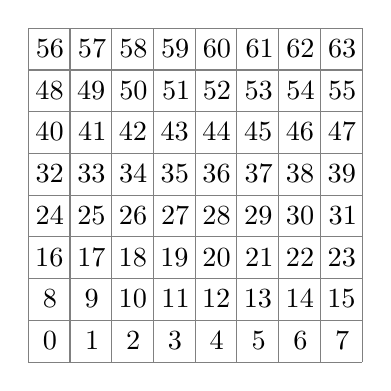
\begin{tikzpicture}[baseline]
			\def\x{0.53}
			\draw[xstep=\x cm,ystep=\x cm,color=gray] (0,0) grid (\x*8,\x*8);
			\matrix[matrix of nodes,
			% http://tex.stackexchange.com/questions/15093/single-ampersand-used-with-wrong-catcode-error-using-tikz-matrix-in-beamer
			ampersand replacement=\&,
			inner sep=0pt,
			anchor=south west,
			nodes={inner sep=0pt,text width=\x cm,align=center,minimum height=\x cm}
			]{
				56	\& 57 \&	58 \& 59 \& 60 \& 61 \& 62 \& 63 \\
				48	\& 49 \&	50 \& 51 \& 52 \& 53 \& 54 \& 55 \\
				40	\& 41 \&	42 \& 43 \& 44 \& 45 \& 46 \& 47 \\
				32	\& 33 \&	34 \& 35 \& 36 \& 37 \& 38 \& 39 \\
				24	\& 25 \&	26 \& 27 \& 28 \& 29 \& 30 \& 31 \\
				16	\& 17 \&	18 \& 19 \& 20 \& 21 \& 22 \& 23 \\
				8	\& 9  \&	10 \& 11 \& 12 \& 13 \& 14 \& 15 \\
				0	\& 1  \&	2  \& 3  \& 4  \& 5  \& 6  \& 7  \\
			};
		\end{tikzpicture}
		\label{fig:mapping}
	}
	\captionof{figure}{Our original chess board with our chosen mapping.}
	\label{fig:chess board and mapping}
\end{figure}
%
Lets take a look at our first real example, where we want to represent all of the white pawns from the initial position.
%
\begin{figure}[H]
	\centering
	\subfloat[Our chess board.]{
	\setchessboard{showmover=false, clearboard, smallboard}
	\def\initialpawns{Pa2, Pb2, Pc2, Pd2, Pe2, Pf2, Pg2, Ph2}
	\chessboard[setpieces=\initialpawns]
	}
	\subfloat[Bitboard representing intial white pawns.]{
		% http://tex.stackexchange.com/questions/12856/tikz-finite-grid-with-character-in-each-cell
		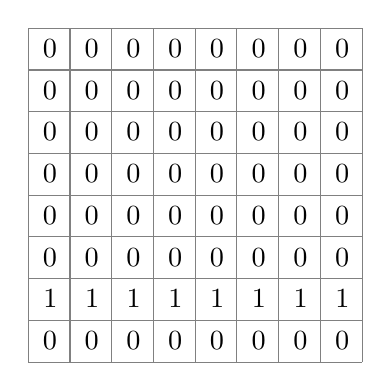
\begin{tikzpicture}[baseline]
		\def\x{0.53}
		\draw[xstep=\x cm,ystep=\x cm,color=gray] (0,0) grid (\x*8,\x*8);
		\matrix[matrix of nodes,
		% http://tex.stackexchange.com/questions/15093/single-ampersand-used-with-wrong-catcode-error-using-tikz-matrix-in-beamer
		ampersand replacement=\&,
		inner sep=0pt,
		anchor=south west,
		nodes={inner sep=0pt,text width=\x cm,align=center,minimum height=\x cm}
		]{
			0 \& 0 \& 0 \& 0 \& 0 \& 0 \& 0 \& 0 \\
			0 \& 0 \& 0 \& 0 \& 0 \& 0 \& 0 \& 0 \\
			0 \& 0 \& 0 \& 0 \& 0 \& 0 \& 0 \& 0 \\
			0 \& 0 \& 0 \& 0 \& 0 \& 0 \& 0 \& 0 \\
			0 \& 0 \& 0 \& 0 \& 0 \& 0 \& 0 \& 0 \\
			0 \& 0 \& 0 \& 0 \& 0 \& 0 \& 0 \& 0 \\
			1 \& 1 \& 1 \& 1 \& 1 \& 1 \& 1 \& 1 \\
			0 \& 0 \& 0 \& 0 \& 0 \& 0 \& 0 \& 0 \\
		};
		\end{tikzpicture}
	}
	\captionof{figure}{The bitboard representing all of the initial white pawns.}
	\label{fig:intial white pawns and bitboard}
\end{figure}
%
The bitboard for all the initial white pawns is as follows:
%
\begin{center}
	\texttt{0000000011111111000000000000000000000000000000000000000000000000}
\end{center}
%
Lets recall some information regarding the chess board square identification and the mapping.
By using a specific mapping, we explicitly assign a direct bit index to each position of the board. So:
%
\begin{alignat*}{3}
A1 &= 0  & \quad G7 &&= 54 \\
B1 &= 1  & H7 &&= 55 \\
C1 &= 2  & A8 &&= 56 \\ 
D1 &= 3  & B8 &&= 57 \\
E1 &= 4  & C8 &&= 58 \\
F1 &= 5  & D8 &&= 59 \\ 
G1 &= 6  & E8 &&= 60 \\
H1 &= 7  & F8 &&= 61 \\
A2 &= 8  & G8 &&= 62 \\ 
B2 &= 9  & H8 &&= 63 \\
\dots& & &
\end{alignat*}
%
But we also explicitly assign a bit index to each position on the board:
%
\begin{alignat*}{1}
0 &= A1\\
1 &= B1\\
\dots\\
62 &= G8\\
63 &= H8\\
\end{alignat*}
%
In general we call such a mapping a \textbf{square mapping}.
We can create a square mapping based on couple of considerations:
%
\begin{itemize}
	\item \textbf{Little-Endian}
	%
	\begin{itemize}
		\item \textbf{Files}: File index 0 maps the A-File, index 7 the H-File.
		\item \textbf{Ranks}: Rank index 0 maps the first Rank, index 7 the eight Rank.
	\end{itemize}
	%
	\item \textbf{Big-Endian}
	%
	\begin{itemize}
		\item \textbf{Files}: File index 0 maps the H-File, index 7 the A-File.
		\item \textbf{Ranks:} Rank index 0 maps the eight Rank, index 7 the first Rank.
	\end{itemize}
	%
\end{itemize}
%
Although you probably noticed that our mapping is a little-endian square mapping,
we can easily deduct this by ourselves by enumerating files and ranks from 0 to 7 each.
There are two common approaches to calculate the square-index from file or rank:
Least Significant File Mapping (LSFM) or Least Significant Rank Mapping (LSRM).
For each of these approaches, we can calculate the square index (as indicated by our mapping) as follows:
%
\begin{minted}{c}
LSF squareIndex = 8*rankIndex + fileIndex
LSR squareIndex = 8*fileIndex + rankIndex
\end{minted}
%
More common is the LSF-mapping where ranks are aligned to the eight consecutive bytes of a bitboard.
Lets try to verify which mapping we just considered. For square \textit{e3}, we know the square index should be equal to 20:
%
\begin{itemize}
	\item LSF squareIndex = $8\cdot \text{rankIndex} + \text{fileIndex} = 8 \cdot 2 + 4 = 20$.
\end{itemize}
%
As we can see in the calculation, we used a rank index of 2 and a file index of 4.
Because the equality holds, we can conclude that we use a little-endian rank-mapping.
In general, we most often use little-endian file-mapping with the A-File addressed by index zero and the H-file addressed by index seven.
In C++, an enumeration of this rank-mapping might look like this:
%
\begin{minted}{C++}
enum enumRank {
er1stRank = 0,
er2ndRank = 1,
er3rdRank = 2,
er4thRank = 3,
er5thRank = 4,
er6thRank = 5,
er7thRank = 6,
er8thRank = 7,
};
\end{minted}
%
The Little-Endian Rank-File (LERF) mapping implies the following C++ enumeration:
%
\begin{minted}{C++}
enum enumSquare {
a1, b1, c1, d1, e1, f1, g1, h1,
a2, b2, c2, d2, e2, f2, g2, h2,
a3, b3, c3, d3, e3, f3, g3, h3,
a4, b4, c4, d4, e4, f4, g4, h4,
a5, b5, c5, d5, e5, f5, g5, h5,
a6, b6, c6, d6, e6, f6, g6, h6,
a7, b7, c7, d7, e7, f7, g7, h7,
a8, b8, c8, d8, e8, f8, g8, h8
};
\end{minted}
%
Below are some bitboards constants that apply to the LERF mapping.
You can convert each of the hexadecimals to binary, probably converting the hexadecimal to a decimal first.
When you convert the hexadecimal to binary, remember that the bit on the left will be the LSB bit, as we decided to use the little-endian format.
When you have eventually converted the hexadecimal to binary, format the binary number as our mapping (\Cref{fig:mapping}) states.
%
\begin{minted}{C++}
a-file             0x0101010101010101
h-file             0x8080808080808080
1st rank           0x00000000000000FF
8th rank           0xFF00000000000000
a1-h8 diagonal     0x8040201008040201
h1-a8 antidiagonal 0x0102040810204080
light squares      0x55AA55AA55AA55AA
dark squares       0xAA55AA55AA55AA55
\end{minted}
%
For example, the hexadecimal for the a-file, \texttt{0x0101010101010101} converted to decimal gives the number 72340172838076673. If we convert this number to binary (little-endian representation), we get the following bitboard:
%
\begin{center}
	\texttt{100000001000000010000000100000001000000010000000100000001}
\end{center}
%
As you can see, the total length of this bit string is not 64: we are missing the padding zeros after the MSB bit.
If we pad the binary number with zeros till it has a length of 64 bits, it will look as follows:
%
\begin{center}
	\texttt{1000000010000000100000001000000010000000100000001000000010000000}
\end{center}
%
Formatting the bitboard according to our representation gives us:
%
\begin{figure}[H]
	\centering
	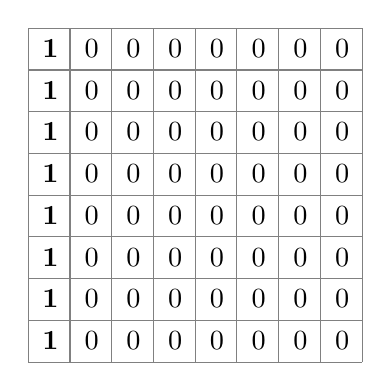
\begin{tikzpicture}[baseline]
	\def\x{0.53}
	\draw[xstep=\x cm,ystep=\x cm,color=gray] (0,0) grid (\x*8,\x*8);
	\matrix[matrix of nodes,
	% http://tex.stackexchange.com/questions/15093/single-ampersand-used-with-wrong-catcode-error-using-tikz-matrix-in-beamer
	ampersand replacement=\&,
	inner sep=0pt,
	anchor=south west,
	nodes={inner sep=0pt,text width=\x cm,align=center,minimum height=\x cm}
	]{
		\textbf{1} \& 0 \& 0 \& 0 \& 0 \& 0 \& 0 \& 0 \\
		\textbf{1} \& 0 \& 0 \& 0 \& 0 \& 0 \& 0 \& 0 \\
		\textbf{1} \& 0 \& 0 \& 0 \& 0 \& 0 \& 0 \& 0 \\
		\textbf{1} \& 0 \& 0 \& 0 \& 0 \& 0 \& 0 \& 0 \\
		\textbf{1} \& 0 \& 0 \& 0 \& 0 \& 0 \& 0 \& 0 \\
		\textbf{1} \& 0 \& 0 \& 0 \& 0 \& 0 \& 0 \& 0 \\
		\textbf{1} \& 0 \& 0 \& 0 \& 0 \& 0 \& 0 \& 0 \\
		\textbf{1} \& 0 \& 0 \& 0 \& 0 \& 0 \& 0 \& 0 \\
	};
	\end{tikzpicture}
	\label{listing:a-file highlight} 
\end{figure}
%
In our representation, this is exactly the \texttt{a}-file being highlighted!
Check the other hexadecimals for yourself!
Now, one final example.
Assume we have our chessboard as show in \Cref{listing:a-file highlight}.
Lets say we want to highlight the \texttt{b}-file, except for \texttt{b8}. The bit at \texttt{a8} has index square 56. We want to move it to 49. As we can see, this would shift the bits from MSB to the LSB. Recall that this is \textbf{RSHFT} with $56-49 = 7$ bits. By essentially performing \texttt{0x0101010101010101} $>>$ 7, we get the desired result (verify this yourself!).
Some notes:
%
\begin{itemize}
	\item Endianness only matters when printing the bitboard.
	When we want to print a bitboard, we need to access the individual bits in the 64-bit unsigned integer.
	By accessing the individual bits in memory, we also have to deal with the way values are stored in memory (internal representation).
	To do this correctly, we need to figure out which representation is currently being used (little-endian or big-endian).
	Note that endianness only matters for the layout of data in memory.
	As soon as data is loaded by the processor to be operated on, endianness is completely irrelevant.
	Shifts, bitwise operations, and so on perform as you would expect (data logically laid out as low-order bit to high) regardless of endianness.
	This means, for example, that the $>>$ operator always shifts the bits towards the LSB, and that the $<<$ operator always shifts the bits towards the MSB.
	
	\item When converting an hex to binary, C++ tends to print the binary in reversed order. You have to watch out for this!
\end{itemize}
%
\begin{code}
\input{"code examples"/"LERF constants"}
\captionof{listing}{Code Snippit for showing the binary number of the given HEX constants that apply to a Little-Endian Rank-File (LERF) mapping.}
\end{code}

\input{sections/"common bitboards"}
\input{sections/"move generation"}


\bibliographystyle{plain}
\bibliography{references/References}
 
\end{document}